% This file was converted to LaTeX by Writer2LaTeX ver. 1.0.2
% see http://writer2latex.sourceforge.net for more info
\documentclass[a4paper]{article}
\usepackage[utf8]{inputenc}
\usepackage[T3,T1]{fontenc}
\usepackage[english]{babel}
\usepackage[noenc]{tipa}
\usepackage{tipx}
\usepackage[geometry,weather,misc,clock]{ifsym}
\usepackage{pifont}
\usepackage{eurosym}
\usepackage{amsmath}
\usepackage{wasysym}
\usepackage{amssymb,amsfonts,textcomp}
\usepackage{color}
\usepackage{array}
\usepackage{hhline}
\usepackage{hyperref}
\hypersetup{pdftex, colorlinks=true, linkcolor=blue, citecolor=blue, filecolor=blue, urlcolor=blue, pdfsubject=, pdfkeywords=}
\usepackage[pdftex]{graphicx}
% List styles
\newcommand\liststyleLSi{%
\renewcommand\labelitemi{\ding{108}}
\renewcommand\labelitemii{o}
\renewcommand\labelitemiii{{\FilledSmallSquare}}
\renewcommand\labelitemiv{\ding{108}}
}
\newcommand\liststyleLSii{%
\renewcommand\labelitemi{\ding{108}}
\renewcommand\labelitemii{o}
\renewcommand\labelitemiii{{\FilledSmallSquare}}
\renewcommand\labelitemiv{\ding{108}}
}
% Page layout (geometry)
\setlength\voffset{-1in}
\setlength\hoffset{-1in}
\setlength\topmargin{0.9839in}
\setlength\oddsidemargin{1.1811in}
\setlength\textheight{9.7251in}
\setlength\textwidth{5.9059in}
\setlength\footskip{0.0cm}
\setlength\headheight{0cm}
\setlength\headsep{0cm}
% Footnote rule
\setlength{\skip\footins}{0.0469in}
\renewcommand\footnoterule{\vspace*{-0.0071in}\setlength\leftskip{0pt}\setlength\rightskip{0pt plus 1fil}\noindent\textcolor{black}{\rule{0.25\columnwidth}{0.0071in}}\vspace*{0.0398in}}
% Pages styles
\makeatletter
\newcommand\ps@Standard{
  \renewcommand\@oddhead{}
  \renewcommand\@evenhead{}
  \renewcommand\@oddfoot{}
  \renewcommand\@evenfoot{}
  \renewcommand\thepage{\arabic{page}}
}
\makeatother
\pagestyle{Standard}
\date{}
\begin{document}
\clearpage\setcounter{page}{1}\pagestyle{Standard}
{\centering 

\includegraphics[width=3.5693in,height=1.7807in]{UFSCar20Summer20Tour-img/UFSCar20Summer20Tour-img1.png}
\par}


\bigskip


\bigskip


\bigskip


\bigskip

{\centering\color{black}
\textbf{UFSCar Summer Tour}
\par}


\bigskip


\bigskip


\bigskip


\bigskip

{\raggedleft\color{black}
Antonio Carlos Falcão Petri 586692
\par}

{\raggedleft\color{black}
José Antônio dos Santos Júnior 586765
\par}

{\raggedleft\color{black}
José Vitor de Carvalho Aquino 609170
\par}

{\raggedleft\color{black}
Tiago Bonadio Badoco 586722
\par}


\bigskip


\bigskip


\bigskip


\bigskip


\bigskip


\bigskip


\bigskip


\bigskip


\bigskip


\bigskip


\bigskip


\bigskip

{\centering\color{black}
São Carlos
\par}

{\centering\color{black}
Junho/2015
\par}

{\color{black}
\textbf{Autores:}}

{\color{black}
Antonio Carlos Falcão Petri
(\href{mailto:falcaopetri@gmail.com}{falcaopetri}\href{mailto:falcaopetri@gmail.com}{@}\href{mailto:falcaopetri@gmail.com}{gmail}\href{mailto:falcaopetri@gmail.com}{.}\href{mailto:falcaopetri@gmail.com}{com})
– Implementação do Jogo}

{\color{black}
José Antônio dos Santos Júnior
(\href{mailto:jusantosjr@hotmail.com}{jusantosjr}\href{mailto:jusantosjr@hotmail.com}{@}\href{mailto:jusantosjr@hotmail.com}{hotmail}\href{mailto:jusantosjr@hotmail.com}{.}\href{mailto:jusantosjr@hotmail.com}{com})
– Desenvolvimento Gráfico}

{\color{black}
José Vitor Aquino
(\href{mailto:jvcaquino95@gmail.com}{jvcaquino}\href{mailto:jvcaquino95@gmail.com}{95@}\href{mailto:jvcaquino95@gmail.com}{gmail}\href{mailto:jvcaquino95@gmail.com}{.}\href{mailto:jvcaquino95@gmail.com}{com})
– Implementação das Estruturas de Dados}

{\color{black}
Tiago Bonadio Badoco
(\href{mailto:tiago.badoco@gmail.com}{tiago}\href{mailto:tiago.badoco@gmail.com}{.}\href{mailto:tiago.badoco@gmail.com}{badoco}\href{mailto:tiago.badoco@gmail.com}{@}\href{mailto:tiago.badoco@gmail.com}{gmail}\href{mailto:tiago.badoco@gmail.com}{.}\href{mailto:tiago.badoco@gmail.com}{com})
- \ Documentação}


\bigskip

{\color{black}
\textbf{Funcionamento do Jogo:}}

{\color{black}
O objetivo do jogo é chegar até determinado ponto do campus da UFSCar de
São Carlos. Para isso o jogador parte do Restaurante Universitário e
sempre tem dois caminhos para seguir o da direita ou o da esquerda.
Cada escolha leva o jogador a um ponto diferente que pode ser um
destino final ou um ponto que lhe proporcione duas novas escolhas.}

{\color{black}
É importante destacar que o jogador não pode voltar no caminho, ou seja,
só pode avançar. Cada caminho para um ponto destino é único, ou seja, o
usuário deve fazer um caminho especifico para vencer. O local de
destino é sorteado de maneira aleatória, toda vez que uma partida é
iniciada.}


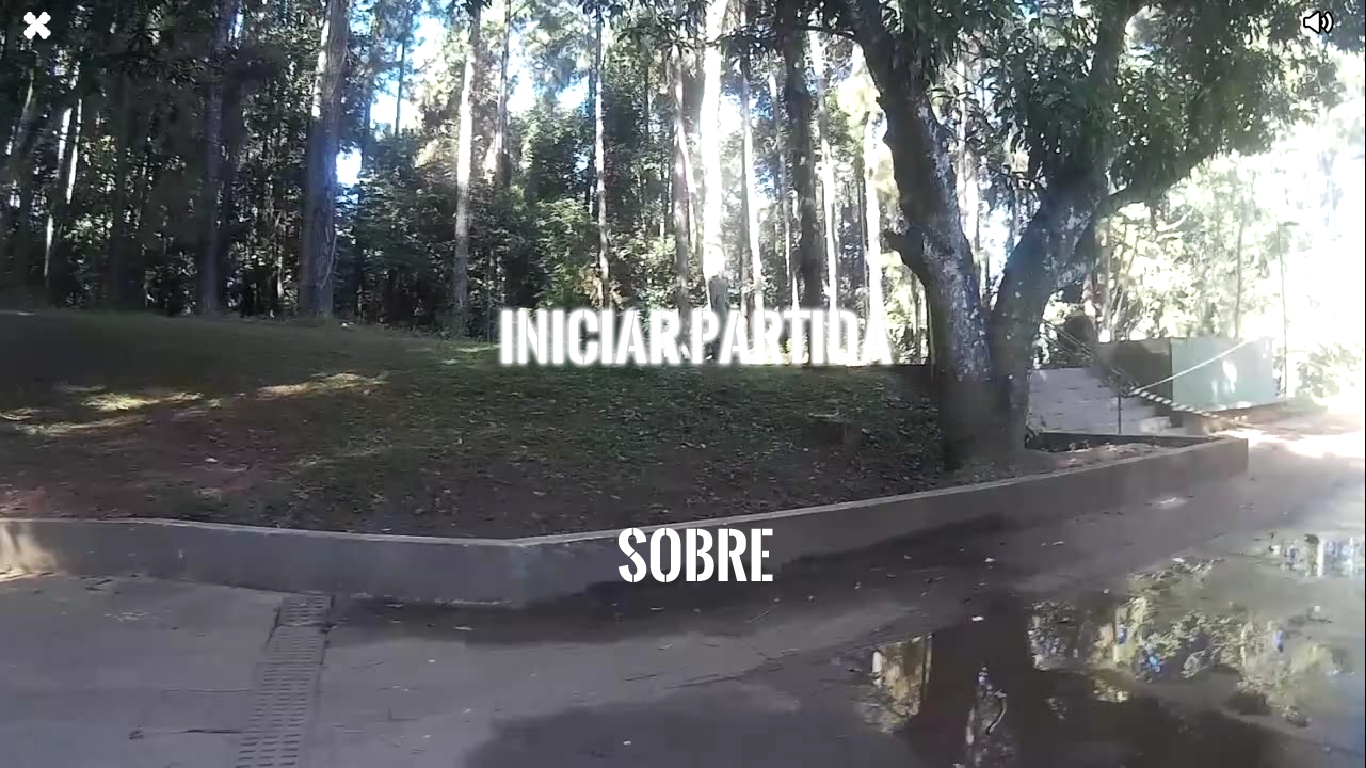
\includegraphics[width=5.9165in,height=3.3335in]{UFSCar20Summer20Tour-img/UFSCar20Summer20Tour-img2.png}


{\centering\color{black}
Imagem 1 - Menu principal
\par}


\bigskip

\clearpage{\color{black}
\textbf{Controles:}}

{\color{black}
Mouse – O mouse controla todas as interações com os menus do jogo,
selecionando as opções desejadas.}

{\color{black}
Seta Esquerda – Seleciona o caminho da esquerda.}

{\color{black}
Seta Direita – Seleciona o caminho da direita.}


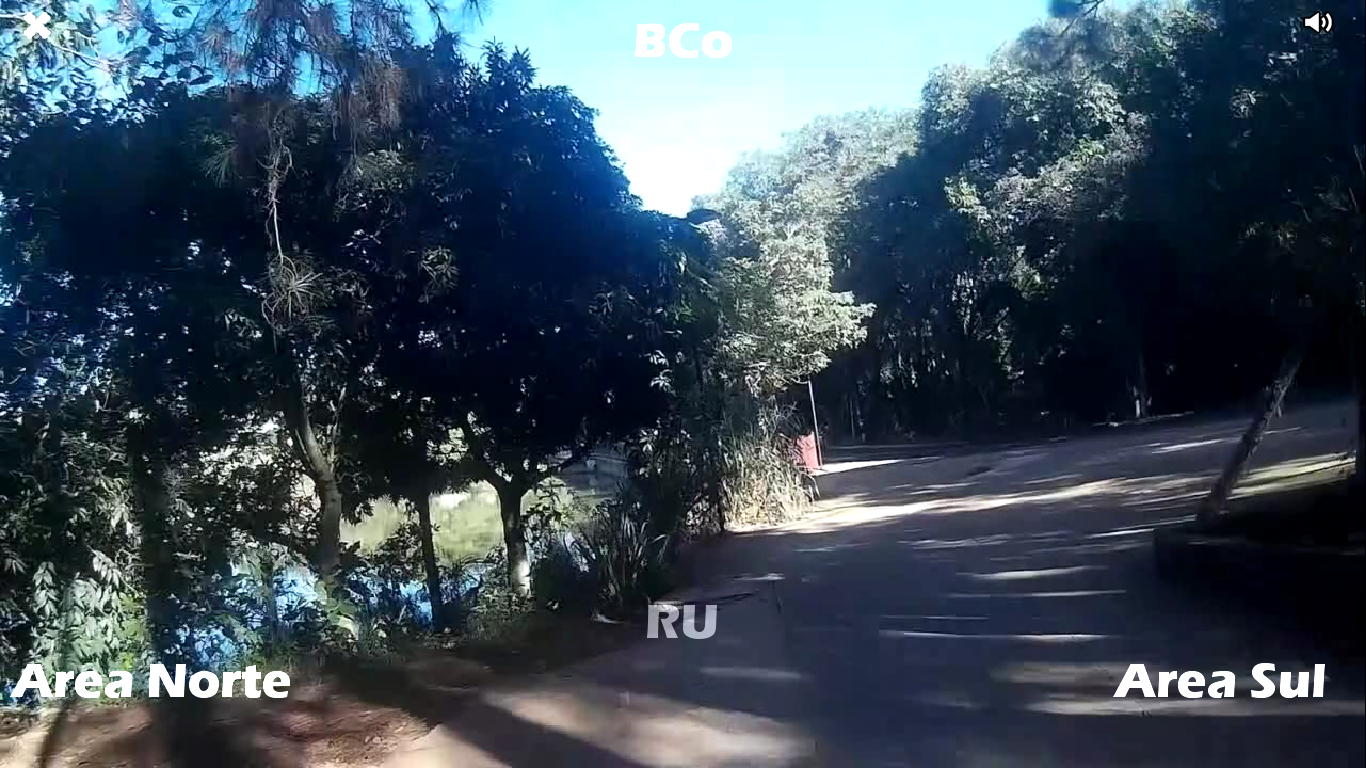
\includegraphics[width=5.9165in,height=3.3335in]{UFSCar20Summer20Tour-img/UFSCar20Summer20Tour-img3.png}


{\centering\color{black}
Imagem 2 - Gameplay
\par}

{\color{black}
\textbf{Ferramentas:}}

\liststyleLSi
\begin{itemize}
\item {\color{black}
Codeblocks;}
\item {\color{black}
Allegro 5.1;}
\item {\color{black}
Photoshop CS5;}
\item {\color{black}
Astah Professional;}
\item {\color{black}
Fruity Loops Producer Edition 11;}
\item {\color{black}
STL, C++~Standard Template Library. }
\end{itemize}

\bigskip

{\color{black}
\textbf{TAD’s}}


\bigskip

{\color{black}
A implementação do jogo utilizada utiliza-se de 2 estruturas de dados
para organizar os principais elementos do jogo, uma Árvore Binária e um
Map.}


\bigskip


\bigskip

\clearpage{\color{black}
\textbf{Como a Árvore é utilizada e implementada?}}

{\color{black}
\ \ A Árvore Binária é definida por um Nó (TreeNode) que guarda um valor
e a uma informação que identifica suas subárvores. Para operar sobre a
Árvore, criou-se uma \textit{friend class} BTUtil, com as manipulações
necessárias para o jogo.}



\begin{center}
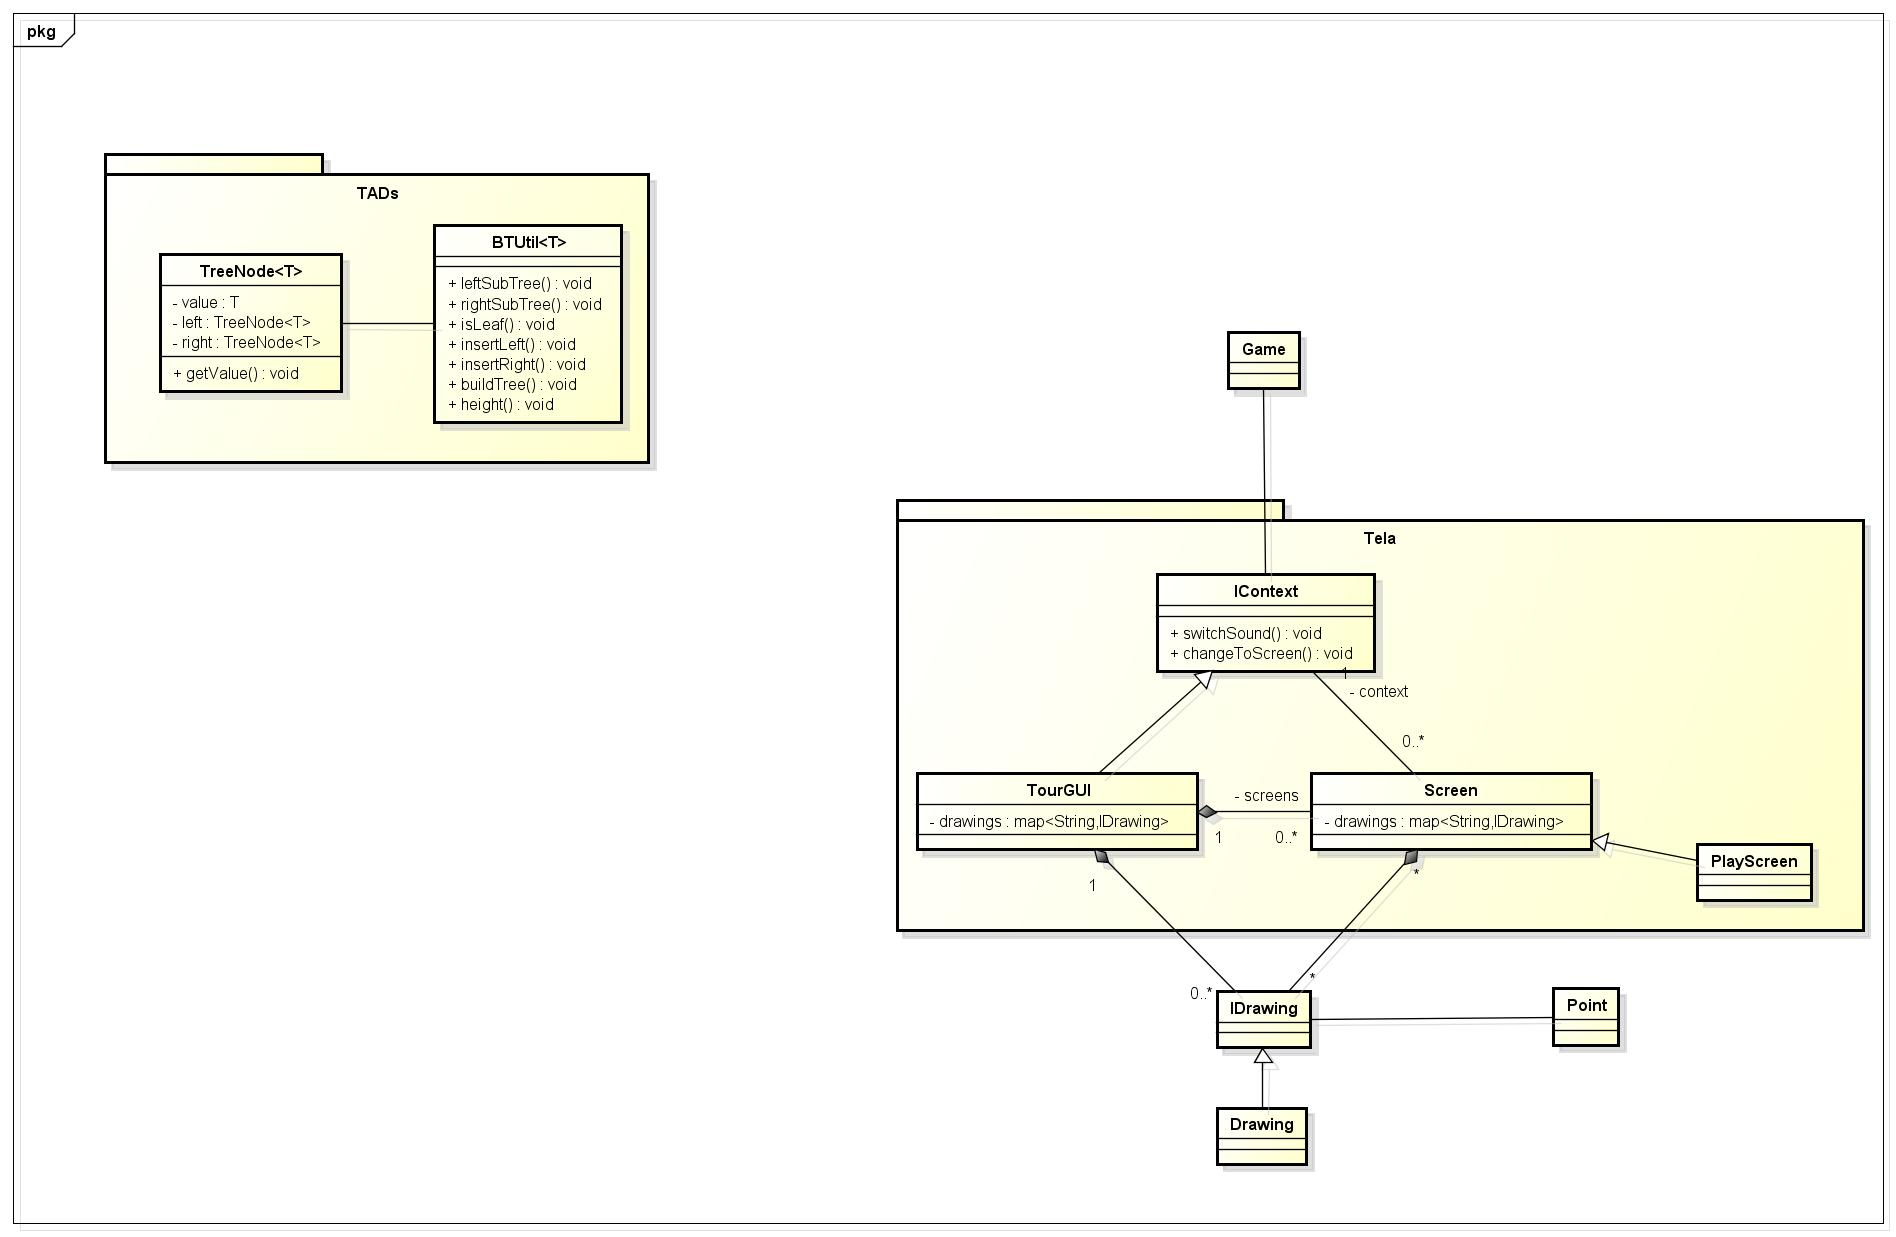
\includegraphics[width=3.8646in,height=2.3228in]{UFSCar20Summer20Tour-img/UFSCar20Summer20Tour-img4.jpg}
\end{center}

\bigskip


\bigskip


\bigskip


\bigskip


\bigskip


\bigskip


\bigskip


\bigskip


\bigskip


\bigskip


\bigskip

{\centering\color{black}
Imagem 3 - Diagrama de Classes: Árvore Binária
\par}


\bigskip


\bigskip

{\color{black}
\textbf{Como o Mapa é utilizado?}}

{\color{black}
Um Mapa é uma estrutura de dados que permite o armazenamento de
elementos “indexados” por uma chave, normalmente única. Externamente, e
para fins didáticos, se parece com um vetor que, ao invés de ter
índices numéricos e acessar o elemento “na posição I”, permite ter
qualquer tipo de objeto como índice e acessa o elemento “com a chave
K”.}

{\color{black}
Internamente, entretanto, os mapas possuem comportamentos diferentes.
Eles costumam ordenar seus dados em relação à chave e, para manter
eficiência nas operações de inserção, consulta e remoção, são
implementados com árvores binárias balanceadas.}

{\color{black}
Na implementação desse jogo, foi utilizado o std::map, um container da
STL. Dessa forma, pode-se definir identificadores às imagens utilizadas
e manipuladas pelo jogo. São utilizados dois maps. Um relaciona o
identificador da imagem ao endereço (relative-path) de seu arquivo no
sistema. O outro, relaciona um identificador (o mesmo, por comodidade e
coerência) à um objeto da Classe IDrawing.}

{\color{black}
Dessa forma, reúne-se todas as imagens do sistema em uma única estrutura
de dados, que assegura velocidade na manipulação desses objetos. Ex:}

{\color{black}
\textcolor[rgb]{0.8392157,0.6156863,0.52156866}{systemImages[}\textcolor[rgb]{0.3372549,0.6117647,0.8392157}{”name”}\textcolor[rgb]{0.8392157,0.6156863,0.52156866}{].}\textcolor[rgb]{0.3254902,0.5058824,0.20784314}{getBitmap}\textcolor[rgb]{0.8392157,0.6156863,0.52156866}{();}}


\bigskip


\bigskip


\bigskip

{\color{black}
\textbf{Arquitetura do Software: }}

{\color{black}
A disposição geral do jogo baseia-se de criação de uma TourGUI, que
encapsula tanto as regras do jogo (Game) quanto a interpretação gráfica
dada a ele. Para tal, criou-se o conceito de Telas (Screens), que
possuem um sub-conjunto de imagens desenháveis.}

{\color{black}
\ \ Dessa forma, não é necessário identificar qual Tela atual está sendo
exibida, pois todas possuem a mesma interface (de métodos). A Tela do
Jogo (PlayScreen), por possuir uma lógica de funcionamento
diferenciada, é uma especialização de uma Screen.}

\begin{center}
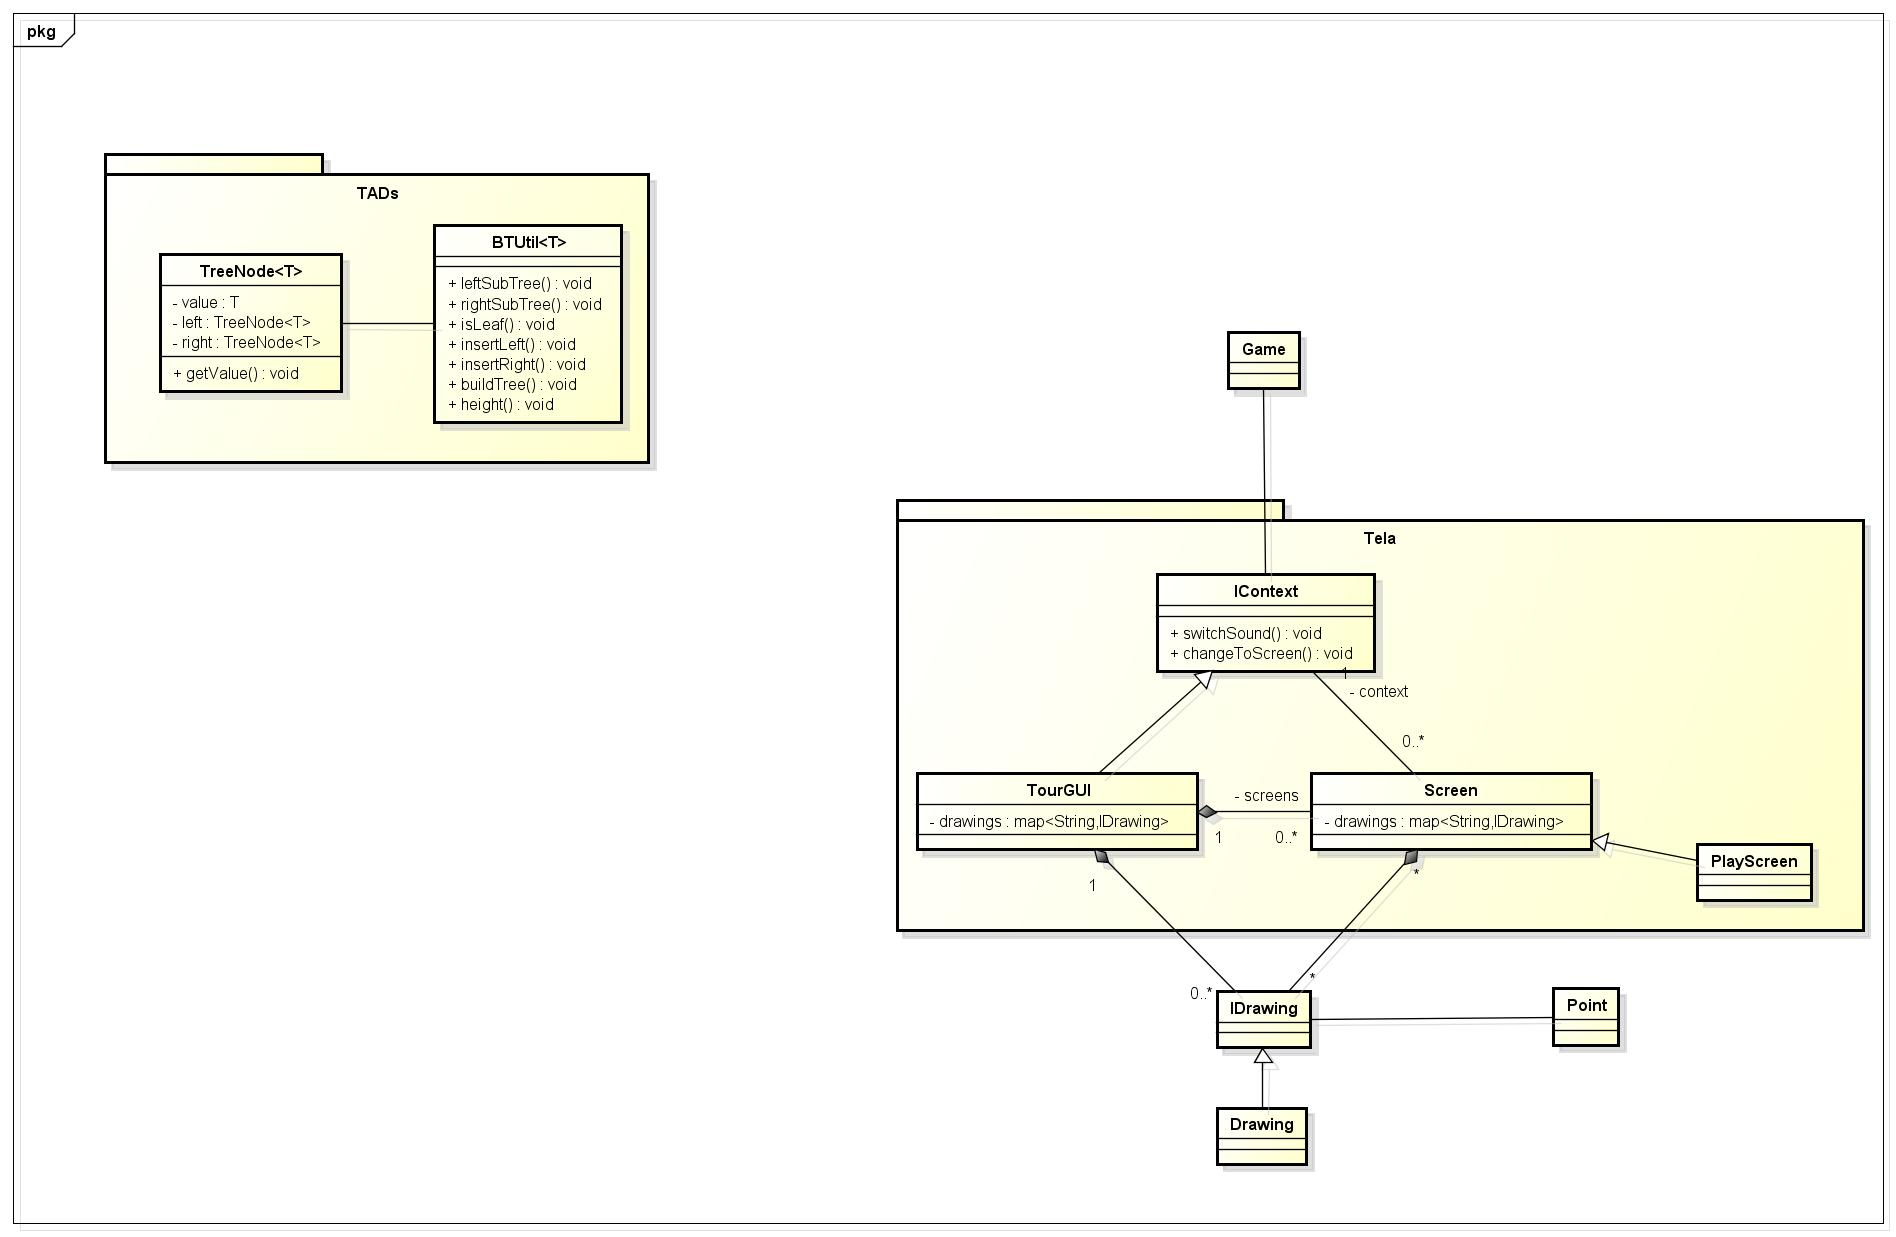
\includegraphics[width=4.9839in,height=4.3283in]{UFSCar20Summer20Tour-img/UFSCar20Summer20Tour-img5.jpg}
\end{center}

\bigskip

{\centering\color{black}
Imagem 4 - Diagrama de Classes: Visão simplificada do Jogo
\par}


\bigskip

{\color{black}
\textbf{Observações e Comentários:}}

{\color{black}
Essa seção reúne pequenas informações quanto ao processo de
desenvolvimento do jogo.}

\liststyleLSii
\begin{itemize}
\item {\color{black}
Para atribuir um ícone ao executável, seguiu-se o procedimento descrito
em
\href{https://www.allegro.cc/forums/thread/601721Monolith}{https}\href{https://www.allegro.cc/forums/thread/601721Monolith}{://}\href{https://www.allegro.cc/forums/thread/601721Monolith}{www}\href{https://www.allegro.cc/forums/thread/601721Monolith}{.}\href{https://www.allegro.cc/forums/thread/601721Monolith}{allegro}\href{https://www.allegro.cc/forums/thread/601721Monolith}{.}\href{https://www.allegro.cc/forums/thread/601721Monolith}{cc}\href{https://www.allegro.cc/forums/thread/601721Monolith}{/}\href{https://www.allegro.cc/forums/thread/601721Monolith}{forums}\href{https://www.allegro.cc/forums/thread/601721Monolith}{/}\href{https://www.allegro.cc/forums/thread/601721Monolith}{thread}\href{https://www.allegro.cc/forums/thread/601721Monolith}{/601721}\href{https://www.allegro.cc/forums/thread/601721Monolith}{Monolith};}
\item {\color{black}
Utilizou-se a função setResourceArchive() no arquivo TheLastTooFast.cpp.
Tal função está descrita em
\href{https://www.allegro.cc/forums/thread/614268}{https}\href{https://www.allegro.cc/forums/thread/614268}{://}\href{https://www.allegro.cc/forums/thread/614268}{www}\href{https://www.allegro.cc/forums/thread/614268}{.}\href{https://www.allegro.cc/forums/thread/614268}{allegro}\href{https://www.allegro.cc/forums/thread/614268}{.}\href{https://www.allegro.cc/forums/thread/614268}{cc}\href{https://www.allegro.cc/forums/thread/614268}{/}\href{https://www.allegro.cc/forums/thread/614268}{forums}\href{https://www.allegro.cc/forums/thread/614268}{/}\href{https://www.allegro.cc/forums/thread/614268}{thread}\href{https://www.allegro.cc/forums/thread/614268}{/614268},
e faz com que o working-directory da aplicação seja mudado para a pasta
em que se encontra o executável. Assim, pode-se utilizar relative-paths
para referenciar os arquivos usados pelo jogo;}
\item {\color{black}
A Arquitetura de Screens proposta não foi suficiente para a
representação abstrata de uma Tela, tendo-se que criar artifícios
internos para a correta manipulação dos elementos. De toda forma, ela
pode ser revista e refinada, possivelmente, enquadrando-a em um Design
Pattern.}
\item {\color{black}
De fato, tal abordagem permitiu um maior reúso do código central do
jogo: o Trabalho 2, Tra1n, que também utiliza-a, foi facilmente
adaptado para gerar esse outro jogo;}
\item {\color{black}
Foi utilizado o Allegro 5.1, a primeira versão da biblioteca a ter
suporte à reprodução de vídeos. Para tal, foi necessário muita pesquisa
e testes experimentais, uma vez que essa versão do Allegro ainda está
em desenvolvimento. Esse fato, aliás, pode acarretar em pequenos
problemas durante a reprodução dos vídeos.}
\end{itemize}

\bigskip
\end{document}
